% TODO: Replace $A$, $B$ with $\alpha$, $\beta$?
% TDOO: Add several sentences about two scales.
% TODO: $A + B \cos 2x$ -> $A + \cos 2x$.
\documentclass[candidate, href, colorlinks]{disser}

\usepackage [T2A] {fontenc}
\usepackage [utf8] {inputenc}
\usepackage [russian, main = english] {babel}
\usepackage {tabularx}

\usepackage [intlimits] {amsmath}
\usepackage {amssymb}
\usepackage {amsfonts}
\usepackage [autostyle] {csquotes}
\usepackage {xcolor}
\usepackage {fancyhdr}
\usepackage {amsthm}
\usepackage {algorithm}
\usepackage {algorithmic}
\usepackage {mathrsfs}
\usepackage {physics}
\usepackage {caption}

\usepackage[a4paper, mag=1000, left=2.5cm, right=1cm, top=2cm, bottom=2cm, headsep=0.7cm, footskip=1cm] {geometry}

\usepackage[style=gost-numeric, backend=biber, language=auto, hyperref=auto, autolang=other, defernumbers, sorting=none]{biblatex}

\addbibresource{bibliography.bib}

\pagestyle{footcenter} % page number at bottom center

\renewcommand*{\thefootnote}{[\arabic{footnote}]}

\captionsetup[algorithm]{
  labelfont = bf,
  labelsep = period
}

\makeatletter
\renewcommand{\ALG@name}{Algorithm}
\makeatother

\newtheorem{proposition}{Proposition}

\begin{document}

% -------------------- TITLE -------------------- %
\begin{titlepage}
\thispagestyle{empty}
\enlargethispage{1cm}
\vspace*{-2cm}

\begin{center}
	Institute of Mathematics with Computing Centre \\ UFRC RAS
\end{center}

\vskip1cm
	
\begin{flushright}
	\emph{As a manuscript}
\end{flushright}
	
\vskip3cm

\begin{center}
	{\large Lebedev Mikhail Evgenievich}
	\vskip1cm
	{\Large\bfseries Bose--Einstein Condensate in Nonlinear Lattices: \\ Mathematical and Numerical Study\par}
	\vskip1.5cm
	{DISSERTATION SUMMARY \\ for the purpose of obtaining academic degree \\ Doctor of Philosophy in Applied Mathematics HSE}
\end{center}

\vskip2cm

\hspace{8cm}\begin{minipage}{0.4\linewidth}
	Academic supervisor \\
	Ph. D. of Technical Sciences \\
	Alfimov Georgy Leonidovich
\end{minipage}

\vfill

\begin{center}
	{Moscow -- \the\year}
\end{center}

\normalfont\clearpage
\end{titlepage}
% -------------------- END -------------------- %

% ---------- GENERAL INFORMATION PAGE --------- %
%\addtocounter{page}{1}
%\thispagestyle{empty}
%\vspace*{-2cm}
%\noindent
%\begin{center}
%Работа выполнена в \emph{ИМВЦ УФИЦ РАН}.
%\end{center}
%\vskip1ex\noindent
%\begin{tabularx}{\linewidth}{@{}lX@{}}
%	\textbf{Научный руководитель:} & \textbf{Алфимов Георгий Леонидович}\\
%	& доктор физико-математических наук \\[6pt]
%	
%	\textbf{Официальные оппоненты:} & \textbf{\textcolor{red}{фамилия имя отчество}}\\
%	& \textcolor{red}{ученая степень, ученое звание} \\[6pt]
%	& \textbf{\textcolor{red}{фамилия имя отчество}} \\
%	& \textcolor{red}{ученая степень, ученое звание} \\[6pt]
%	
%	\textbf{Ведущая организация:} & Институт математики с вычислительным центром УФИЦ РАН
%\end{tabularx}
%
%\vskip5ex\noindent
%Защита состоится \datefield{} в \rule[0pt]{1cm}{0.5pt} часов
%на заседании диссертационного совета \emph{\textcolor{red}{шифр совета}} при \emph{\textcolor{red}{название организации, при которой создан совет}}, расположенном по адресу: \emph{\textcolor{red}{адрес}}.
%
%\vskip1ex\noindent
%С диссертацией можно ознакомиться в библиотеке \emph{\textcolor{red}{название организации}}, а также по ссылке \href{http://www.xyz.com}{\textcolor{red}{http://www.xyz.com}}.
%
%\vskip1ex\noindent
%Автореферат разослан \datefield{}
%
%\vskip2ex\noindent
%Отзывы и замечания по автореферату в двух экземплярах, заверенные
%печатью, просьба высылать по вышеуказанному адресу на имя ученого секретаря диссертационного совета.
%
%\vfill\noindent
%\begin{minipage}[b]{1\linewidth}
%	Ученый секретарь \\
%	диссертационного совета, \\
%	\emph{кандидат физико-математических наук}, \emph{доцент} \hfill \emph{Самбурский Л. М.}
%\end{minipage}
%
%\clearpage
% -------------------- END -------------------- %

\nsection{General Description of the Work}

\textbf{Introduction.}
Since the 90s of the last century, the Nonlinear Schr\"odinger Equation (NLS) with additional spatial non-autonomous terms has been an object of thorough studies.
Specific interest to this class of equations has been caused by progress in experimental study of Bose-Einstein Condensate (BEC).
Being predicted in 20-ies, this state of matter was obtained for the first time in 1995 independently in experiments of two groups of researchers\footnote{A. Einstein, ``Quantentheorie des einatomigen idealen Gases'', Preussische Akademie der Wissenschaften, Berlin, 1924.}.
In 2001 this discovery was awarded by Nobel Prize.

The ability of the observation of BEC stimulated experimental and theoretical studies all over the world.
These studies opened a variety of different practical applications.
Specifically, it's expected that the usage of BEC may have a huge impact on the development of the new high-frequency interferometers.\footnote{C. Gross, T. Zibold, E. Nicklas, J. Esteve, and M. K. Oberthaler, ``Nonlinear atom interferometer surpasses classical precision limit'', Nature, Vol. 464, P. 1165--1169, 2010.}.
BEC can be used in quantum computers industry\footnote{D. Jaksch, P. Zoller, ``The cold atom Hubbard toolbox'', Annals of Physics, Vol. 315, P. 52--79, 2005.}, and in quantum lasers as well\footnote{W. Guerin, J.-F. Riou, J. P. Gaebler, V. Josse, P. Bouyer, and A. Aspect, ``Guided Quasicontinuous Atom Laser'', Phys. Rev. Lett., Vol. 97, P. 200402, 2006.}.

It turn out that the dynamics of elongated BEC in so-called mean-field approximation is well described by the Sr\"odinger type equation with spatial non-autonomous terms,
\begin{equation}
	i \Psi_t + \Psi_{xx} - U(x) \Psi + P(x) |\Psi^2| \Psi = 0.
\label{eq:gpe}
\end{equation}
In the context of BEC equation \eqref{eq:gpe} is called {\it Gross--Pitaevskii equation} (GPE).
Here $\Psi(t, x)$ is the dimensionless wave function of the condensate cloud, that is assumed to be elongated along the axis $x$.
Function $U(x)$ describes the trap potential that is used to confine BEC, and $P(x)$ corresponds to nonlinear potential (also called {\it pseudopotential}).
The pseudopotential describes the dependence of scattering length on the coordinates that may be non-constant due to various reasons.
Possible experimental techniques to achieve non-constant scattering length involves optical or magnetic Feshbach resonances\footnote{C. Chin, R. Grimm, P. Julienne, and E. Tiesinga, ``Feshbach resonances in ultracold gases'', Rev. Mod. Phys. Vol. 82, P. 1225, 2010.}.
Intervals with the positive values of pseudopotential, $P(x) > 0$, correspond to the case of interatomic attraction of the condensate particles, while intervals with negative values, $P(x) < 0$, correspond to the interatomic repulsion.
The prototypical examples of $U(x)$ are the harmonic potential well $U(x) = Ax^2$ (the magnetic trap), periodic potential $U(x) = A \cos 2x$ (the optical trap), and other types of potential wells.


As a model examples of the pseudopotential $P(x)$ the different functions can be used, including periodic ones.
In the latter case one can say that there exists a {\it nonlinear lattice} interacting with the condensate cloud.
In physical experiments nonlinear lattice is created by the resonant action of additional magnetic\footnote{S. Inouye, M. R. Andrews, J. Stenger, H.-J. Miesner, D. M. Stamper-Kurn \& W. Ketterle, ``Observation of Feshbach resonances in a Bose--Einstein condensate'', Nature, Vol. 392, P. 151-154, 1998.} or optical\footnote{L. W. Clark, Li-Chung Ha, Chen-Yu Xu, and Cheng Chin, ``Quantum Dynamics with Spatiotemporal Control of Interactions in a Stable Bose--Einstein Condensate'', Phys. Rev. Lett., Vol. 115, P. 155301, 2015.} field.
The presence of nonlinear lattice may provide additional possibilities for stabilization of the condensate cloud and for exciting new condensate states.
In order to model a nonlinear lattice in theoretical works the cosine pseudopotential of the form $P(x) = A + B \cos \Omega x$ is traditionally used\footnote{\label{note:malomed} H. Sakaguchi,  B. A. Malomed, ``Matter-wave solitons in nonlinear optical lat­tices'', Phys. Rev. E, Vol. 72, P. 046610, 2005.}.

It's also worth noting that similar problems arise in other branches of physics, particularly in nonlinear optics. 
In various optical applications, equation \eqref{eq:gpe} describes propagation of a light beam in an optical fiber.
In this case, periodic spatial modulation of nonlinearity is achieved by adding resonant dopants into the fiber\footnote{J. Hukriede, D. Runde, and D. Kip, ``Fabrication and application of holographic Bragg gratings in lithium niobate channel waveguides'', J. Phys. D, Vol. 36, R1, 2003.}.

For different physical applications solutions of equation \eqref{eq:gpe} of the special form, so-called {\it stationary localized solutions} ({\it stationary localized modes}, SLMs), play an important role.
Such solutions can be obtained by putting into \eqref{eq:gpe} an ansatz
\begin{equation}
	\Psi(t, x) = u(x) e^{-i \omega t},
\label{eq:ansatz}
\end{equation}
where function $u(x)$ satisfies localization conditions of the form:
\begin{equation}
	\lim \limits_{x \to \infty} u(x) = 0.
\label{eq:localization}
\end{equation}
Here $\omega$ is a real parameter that stands for a chemical potential of the condensate.
Profile $u(x)$ of the stationary localized solution is a real-valued function\footnote{G. L. Alfimov, V. V. Konotop, and M. Salerno, ``Matter solitons in Bose--Einstein condensates with optical lattices'', Europhys. Lett., Vol. 58, P. 7--13, 2002}, satisfying an equation
\begin{equation}
	u_{xx} + Q(x) u + P(x) u^3 = 0; \quad Q(x) = \omega - U(x).
\label{eq:stationary}
\end{equation}

It should be noted that not all localized solutions of Eq.~\eqref{eq:stationary} are equally interesting from a physical point of view.
Specifically, stability is one of the critically important property of the localized solutions.
If SLM is unstable, small perturbation of such solution leads to its collapse during the evolution described by equation \eqref{eq:gpe}.
Therefore, stable localized solutions are especially valuable from the perspective of physical applications.
The analysis of stability is an essential part of the theoretical study of SLMs.

\textbf{Formulation of the problem.}
During the study of dynamics described by equation \eqref{eq:gpe} the following questions are naturally arise:
\begin{enumerate}
	\item Is it possible to describe {\it exhaustively all} stationary localized solutions of equation \eqref{eq:gpe} which simultaneously coexist for given parameters?
	\item How to effectively identify stable solutions among them?
\end{enumerate}

\textbf{Some survey of the current state of the field.}
It's worth noting that in majority of works devoted to this topic the problem of finding / describing of {\it all} SLMs is not raised.
Instead, usually only specific classes of solutions corresponding to particular physical structures are described, see a comprehensive review\footnote{Y. V. Kartashov, B. A. Malomed, and L. Torner, ``Solitons in nonlinear lattices'', Rev. Mod. Phys. Vol. 83, P. 247, 2011.}.
At the same time, despite some ``ambition'' of the questions above, the combination of rigorous analytical methods with numerical computations makes it possible to achieve significant progress in this direction.
Let us note some important results.

For equation \eqref{eq:stationary} with potential $U(x)$ of the form of infinite potential well, $U(x) = A x^2$, in the case of repulsive interparticle interactions, $P(x) \equiv -1$, the computational descriptive procedure has been proposed\footnote{\label{note:alfzez} G. L. Alfimov, D. A. Zezyulin, ``Nonlinear modes for the Gross--Pitaevskii equation --- a demonstrative computational approach'', Nonlinearity, Vol. 20, P. 2075--2092, 2007.}.
This procedure provides a computational evidence and can guarantee the exhaustive description of {\it all} bounded solutions of equation for the given set of parameters.
The proposed method was afterwards generalized to systems of several coupled Gross -- Pitaevskii equation, in which the corresponding pseudopotential coefficients do not depend on the spatial coordinate\footnote{G. L. Alfimov, I. V. Barashenkov, A. P. Fedotov, V. V. Smirnov, D. A. Zezyulin, ``Global search for localised modes in scalar and vector nonlinear Schr{\"o}dinger-type equations'', Physica D, Vol. 397, P. 39--53, 2019.}.

It was shown, that for the periodic potential $U(x)$ in the case of repulsive interactions of the condensate particles, $P(x) \equiv -1$, there exist sufficient conditions that again allow to exhaustively describe {\it all} bounded solutions of equation \eqref{eq:stationary}.
Moreover, it was shown that under these conditions there exist one-to-one correspondence between the bounded solutions and all possible bi-infinite sequences of symbols of some finite alphabet\footnote{\label{note:alfavr} G. L. Alfimov, A. I. Avramenko, ``Coding of nonlinear states for the Gross--Pitaevskii equation with periodic potential'', Physica D, Vol. 254, P. 29--45, 2013.}.
Such sequences are called as {\it codes of solutions}, and the process of assigning of such codes as {\it coding of solutions}.
In the above mentioned paper, the verification of the sufficient conditions was performed by means of numerical computations.
Results of this paper were further developed\footnote{G. L. Alfimov, P. P. Kizin, D. A. Zezyulin, ``Gap solitons for the repulsive Gross-Pitaevskii equation with periodic potential: Coding and method for computation'', Discrete and Continuous Dynamical Systems --- Series B, Vol. 22, P. 1207--1229, 2017.}, specifically: there has been proposed an algorithm that allows to numerically reconstruct solution profile by its symbolic code.

It's also worth to mention the mathematical works of F. Zanolin and co-authors\footnote{Ch. Zanini, F. Zanolin, ``Complex Dynamics in One-Dimensional Nonlinear Schr\"odinger Equations with Stepwise Potential'', Complexity, Vol. 2018, Article ID 2101482, 2018.}\textsuperscript{,}\footnote{Ch. Zanini, F. Zanolin, ``An Example of Chaos for a Cubic Nonlinear Schr\"odinger Equation with Periodic Inhomogeneous Nonlinearity'', Advanced Nonlinear Studies, Vol. 12, No. 3, P. 481--499, 2012.}, in which the existence of some types of solutions in related problems is proved.
Such solutions also can be completely described in terms of nonlinear dynamics.
Authors of these works use an approach that relies on topological argumentation.
This approach differs from the one presented in the dissertation.

\textbf{Relevance of research topic.}
Generalization of the above mentioned results to the case of variable pseudopotential, $P(x) \neq \mathrm{const}$, is an actual problem.
Specifically, one of the perspective direction of the research is the generalization of the solution coding framework to the case of periodic pseudopotential.
Detailed classification of solutions of Eq.~\eqref{eq:gpe} opens up the possibility of experimental finding of new, previously unknown stable SLMs.

\textbf{Tasks and objectives of the study.}
Main object of the study in the dissertation is the set of stationary solutions of one-dimensional Gross -- Pitaevskii equation \eqref{eq:gpe} with {\it periodic pseudopotential}.
Tasks and objectives of the study can be formulated as follows:
\begin{enumerate}
	\item Formulate sufficient conditions that allow to generalize method of coding of SLMs\textsuperscript{\ref{note:alfavr}} to the case of periodic pseudopotential; specify the way of verification of these conditions (analytically or with numerical computations).
	\item Study the set of stationary solutions of equation \eqref{eq:gpe} with periodic pseudopotential in the case of essentially nonlinear interactions, when the ordinary potential can be neglected, $U(x) \equiv 0$.
	\item For the case of infinite potential well, $U(x) = A x^2$, investigate the impact of periodic pseudopotential on the structure of the set of stationary localized solutions and their stability.
\end{enumerate}

\textbf{Research methodology and methods.}
For studying of possible types of SLMs the so-called {\it method of excluding of singular solutions}\textsuperscript{\ref{note:alfavr}} is used in the current work.
We call a solution of equation \eqref{eq:stationary} {\it singular} if it goes to infinity at a finite point $x = x_0$ of the real axis, i.e.
\begin{equation}
	\lim \limits_{x \to x_0} u(x) = \infty.
\end{equation}
Obviously, such solutions cannot describe a profile of wave function, so they should be excluded from the consideration.
Under certain conditions, ``most part'' of solutions of Eq.~\eqref{eq:stationary} are singular.
The set of remaining solutions, called {\it regular}, turns out to be quite ``poor'' and it can be fully described in terms of symbolic dynamics.

Numerical solution of differential equation \eqref{eq:stationary} is performed by means of Runge -- Kutta method of the fourth order.
In order to compute profiles of localized solutions of equation \eqref{eq:stationary} the shooting method is used.
The obtained solutions are checked for the linear stability by solving the corresponding eigenvalue problem in the Fourier space (Fourier Collocation Method\footnote{J. Yang, ``Nonlinear Waves in Integrable and Nonintegrable Systems'', Philadelphia: SIAM, 2010.}), and also via the evolutional simulation of dynamics of \eqref{eq:gpe} with a conservative finite-difference scheme\footnote{V. Trofimov, N. Peskov Comparison of finite-difference schemes for the Gross-Pi­ taevskii equation // Mathematical Modelling and Analysis. — 2009. — Mar. — Vol. 14. — P. 109–126.}.
All the algorithms and numerical methods are implemented in {\tt MATLAB} using {\tt MEX} extension for high performance computing support.

\textbf{Scientific novelty.}
In the dissertation work, a number of general propositions about regular and singular solutions of equation \eqref{eq:stationary} have been proven.
These propositions establish conditions under which equation \eqref{eq:stationary} admits the existence of singular solutions, and when all its solutions are regular.
In particular, it was shown that if pseudopotential takes negative value at least at one point $x_0$, $P(x_0) < 0$, then there exist two one-parametric families of solutions which tend to infinity at this point $x_0$.
Asymptotic expansions were also obtained for these families.

The method of excluding of singular solutions was further developed.
The dissertation proposes sufficient conditions of existence of one-to-one correspondence between regular solutions of equation \eqref{eq:stationary} and bi-infinite symbolic sequences over some alphabet. 
In contrasts to the previously obtained results\textsuperscript{\ref{note:alfavr}}, the proposed conditions admit effective numerical verification.
An algorithm of the numerical verification is provided in the dissertation along with its theoretical justification.

For the case $U(x) \equiv 0$ and cosine periodic pseudopotential of the form $P(x) = A + B \cos 2x$ the set of stationary localized solutions has been studied.
With applying the above-mentioned techniques, the set of SLMs was effectively described, and, eventually, new stable localized solution, named {\it dipole soliton} \cite{LebedevAlfimovMalomed}, was revealed.
This solution has been previously unknown while considering problems related to equation \eqref{eq:gpe}.

Finally, in the case of infinite potential well, $U(x) = A x^2$, the impact of periodic pseudopotential of the form $P(x) = A + B \cos \Omega x$ on the set of SLMs was studied.
It was shown that in comparison with well-studied case $P(x) = \mathrm{const}$, the set of stationary localized solutions turns out to be much richer.
Namely, there exist essentially nonlinear solutions which do not exist in the low-amplitude limit.
The dependence of the SLMs stability on the frequency $\Omega$ of the pseudopotential was studied.
For the pseudopotential with zero mean, $P(x) = B \cos \Omega x$, it was found that the increase of frequency $\Omega$ allows to stabilize low-amplitude solutions, whose analogues in the model with $P(x) = \mathrm{const}$ are unstable.

% \textbf{Теоретическая и практическая значимость.}
% Результаты, изложенные в диссертации, могут быть использованы при проведении экспериментов с конденсатом Бозе--Эйнштейна.

\textbf{Key aspects to be defended:}
\begin{enumerate}
	\item General statements on the presence and absence of singular solutions of equation \eqref{eq:stationary} have been proved.
		It was shown that in the case $P(x) > 0$ all solutions of \eqref{eq:stationary} are regular.
		If $P(x)$ is negative at least at one point $x_0$, $P(x_0) < 0$, then there exist two one-parametric families of solutions, which tend to infinity at the point $x_0$.
		The asymptotic behaviour of such families was studied, and the asymptotic series for such families are provided.
		In the case $Q(x) < 0$ and $P(x) < 0$, it was shown that all solutions of equation \eqref{eq:stationary} are singular.
	\item For equation \eqref{eq:stationary} sufficient conditions of the possibility of regular solutions coding were formulated.
		The effective numerical algorithm for their validation was provided as well.
	\item For the case $U(x) \equiv 0$, $P(x) = A + \cos 2x$ the set of SLMs of Eq.~\eqref{eq:gpe} was studied.
		This study revealed new stable localized solution, named {\it dipole soliton}.
	\item For infinite potential well of the form $U(x) = A x^2$ it was shown that the presence of periodic pseudopotential leads to emergence of new classes of SLMs, which have no analogues in models with $P(x) = \mathrm{const}$.
		For the pseudopotential with zero mean, it was found that the frequency of the pseudopotential affects the stability of SLMs significantly.
		Particularly, the increase of the frequency can stabilize low-amplitude localized solutions.
\end{enumerate}

\textbf{Confidence level and approbation of the results.}
The Gross -- Pitaevskii model is a classical model of physics of ultra-cold temperatures and its confidence is beyond doubt.
In dissertation, localized stationary solutions of this model are constructed, and their stability is investigated numerically.
Numerical computation of solutions is performed by means of standard numerical methods with controlled accuracy.
Study of stability of obtained solutions is fulfilled by using of the spectral method which has proven itself in similar problems well.
Results of analysis of stability are verified by numerical evolution in a framework of conservative finite-difference scheme.
The key results of the dissertation were reported at various scientific seminars and conferences, including:
\begin{enumerate}
	\item <<Фундаментальная математика и ее приложения в естествознании>>, BSU, Ufa, September, 2015 y.
	\item ``Dynamics, Bifurcations and Chaos III'', Lobachevsky State University of Nizhni Novgorod, Nizhni Novgorod, July, 2016 y.
	\item ``Complex Analysis, Mathematical Physics and Nonlinear Equations'', Bashkortostan, Bannoe Lake, March, 2018 y.
	\item ``Nonlinear Phenomena in Bose Condensates and Optical Systems'', Tashkent, Uzbekistan, August, 2018 y.
	\item ``Complex Analysis, Mathematical Physics and Nonlinear Equations'', Bashkortostan, Bannoe Lake, March, 2019 y.
	\item ``Complex Analysis, Mathematical Physics and Nonlinear Equations'', Bashkortostan, Bannoe Lake, March, 2021 y.
\end{enumerate}

\textbf{Publications.}
Materials of dissertation were published in 9 printed works, among them there are 3 articles in peer-reviewed journals \cite{AlfimovLebedev, LebedevAlfimovMalomed, AlfimovGegelLebedevMalomedZezyulin}, and 6 abstracts of various conferences \cite{Ufa2015, NizhniNovgorod2016, Bannoe2018, Tashkent2018, Bannoe2019, Bannoe2021}.
During the work on the dissertation, the author also published 2 articles\footnote{M. E. Lebedev, D. A. Dolinina, K. B. Hong, {\it et al.}, ``Exciton-polariton Josephson junctions at finite temperatures'', Scientific Reports Vol. 7, P. 9515, 2017}\textsuperscript{,}\footnote{D. A. Zezyulin, M. E. Lebedev, G. L. Alfimov, and B. A. Malomed, ``Symmetry breaking in competing single-well linear-nonlinear potentials'', Phys. Rev. E, Vol. 98, P. 042209, 2018.} on related topes (results of one of these works were also reported on conference\footnote{D. A. Zezyulin, M. E. Lebedev, G. L. Alfimov, and B. A. Malomed, ``Symmetry breaking in competing single-well linear-nonlinear potentials'', Abstracts of conference ``Complex Analysis, Mathematical Physics and Nonlinear Equations'', Bashkortostan, Bannoe Lake, March, 2019.}).

\textbf{Personal contribution of the author.}
The content of the dissertation and the key aspects submitted for defense reflect the personal contribution of the author to the published works.
Preparation for the publication of the obtained results was carried out jointly with co-authors, and the contribution of the candidate was decisive.
All the results presented in the dissertation were obtained personally by the author using the developed methods and computer programs.

% TODO: fill it!
\textbf{Structure and size of the dissertation.}
The thesis consists of introduction, four chapters, three appendices, and a bibliography.
Total size of the dissertation is \textcolor{red}{?} page.
Among them there are \textcolor{red}{?} pages of text, including \textcolor{red}{?} figures, four tables and one algorithm schema.
Bibliography consists of \textcolor{red}{?} titles on \textcolor{red}{?} pages.

\nsection{Content of the Work}

\textbf{In Introduction} the relevance of the dissertation work is justified, author formulates goal of the research and its novelty is argued.
The practical significance of the obtained results is shown, and scientific aspects submitted for defense are presented.

Main definitions that are related to the object of study are introduced.
{\it Stationary localized solutions} (or {\it stationary localized modes}, SLMs) are defined as solutions of equation \eqref{eq:gpe} of the form \eqref{eq:ansatz} that satisfy the localization conditions \eqref{eq:localization}.
Solutions $u(x)$ of equation \eqref{eq:stationary} is called  {\it singular} if for some finite point $x_0$ the relation $u(x) \to \infty$ as $x \to x_0$ takes place.
Point $x_0$ is called as collapse point for the solution $u(x)$.
One can say that such solution {\it collapses} at the point $x_0$.
On the contrary, solution is called {\it regular} if there is no such point $x_0$.

\textbf{In Chapter I} general propositions about regular and singular solutions of equation \eqref{eq:stationary} are formulated and proved.

\begin{proposition}
\label{prop:absense-of-singular-solutions}
	Let for equation \eqref{eq:stationary} functions $Q(x), \, P(x) \in C^1(\mathbb{R})$, and for all $x \in \mathbb{R}$
	\begin{enumerate}
		\item[(a)] $P(x) \ge P_0 > 0$, $|P'(x)| \le \widetilde{P}$;
		\item[(b)] $Q(x) \ge Q_0$, $|Q'(x)| \le \widetilde{Q}$.
	\end{enumerate}
	Then solution of the Cauchy problem for equation \eqref{eq:stationary} with arbitrary initial condi­tions can be continued to the whole real axis R.
\end{proposition}

Proposition \ref{prop:absense-of-singular-solutions} established conditions of absence of singular solutions.
One of these conditions requires function $P(x)$ to be positive-defined.
On the other hand side, if function $P(x)$ takes a negative value at least at one point $x_0$, $P(x_0) < 0$, then there exist two families of solutions of equation \eqref{eq:stationary} that collapse at this point.
In order to formulate the below-following proposition it's convenient to let $P(x_0) = -1$ (it's always can be achieved by a suitable renormalization).

\begin{proposition}
\label{prop:singular-families}
	Let $\Omega$ be a neighbourhood of the point $x_0$, $Q(x) \in C^2(\Omega)$, and $P(x) \in C^4(\Omega)$.
	Then there exist two $C^1$-smooth one-parametric families of solutions for equation \eqref{eq:stationary}, collapsing at the point $x = x_0$ (while approaching from the left, $x \to x_0{-}0$), and connected by a symmetry $u \to -u$.
	Each of these families can be parametrized by a free variable $C \in \mathbb{R}$, and, moreover, the following asymptotic expansions are valid:
	\begin{equation}
		\pm u(x) = \dfrac{\sqrt{2}}{\eta} + A_0 + A_1 \eta + A_2 \eta^2 + A_3 \eta^3 \ln |\eta| + C \eta^3+ A_4 \eta^4 \ln |\eta| + \dots.
	\label{eq:expansion}
	\end{equation}
	Here $\eta = x - x_0$, and coefficients $A_n$ can be expressed in terms of coefficients $Q_n$, $P_n$ of the corresponding expansions for the functions $Q(x)$, $P(x)$
	\begin{equation}
		Q(x) = Q_0 + Q_1 \eta + Q_2 \eta^2 \dots, \quad P(x) = -1 + P_1 \eta + P_2 \eta^2 + \dots.
	\end{equation}
\end{proposition}

Analogous one-parametric families of collapsing solutions also exist to the right side of the point $x = x_0$.
Finally, in the first chapter, there are established conditions under which equation \eqref{eq:stationary} has no regular solutions at all, except for the zero solution, $u(x) \equiv 0$.

\begin{proposition}
\label{prop:all-solutions-are-singular}
 	Let for all $x \in \mathbb{R}$ the conditions $P(x) \le P_0 < 0$, $Q(x) \le Q_0 < 0$ take place.
 	Then all solutions of equation \eqref{eq:stationary} are singular except for the zero one.
\end{proposition}

One of the consequences of the obtained results is that if pseudopotential $P(x)$ is a sign-altering function then singularity is a common solutions behaviour for equation \eqref{eq:stationary}.
This fact makes it possible to apply method of excluding of singular solutions\textsuperscript{\ref{note:alfavr}}.
Results of the first chapter were published in \cite{AlfimovLebedev} and \cite{Ufa2015}.

\textbf{In Chapter II} the framework of coding of stationary states is introduced for equation \eqref{eq:gpe} with $L$-periodic functions of potential, $U(x + L) = U(x)$, and pseudopotential, $P(x + L) = P(x)$.
It turns out that under certain conditions the set of regular solutions of equation \eqref{eq:stationary} can be fully described accordingly to the structure of the so-called {\it coding sets}: $\mathscr{U}_L^+$, $\mathscr{U}_L^-$, $\mathscr{U}_L$.
These sets are defined on the plane $(u, u')$ of initial conditions for equation \eqref{eq:stationary} as follows.
Set $\mathscr{U}_L^+$ consists of all initial conditions to the Cauchy problem such that the corresponding solutions are bounded on the interval $[0; L]$.
Similarly, set $\mathscr{U}_L^-$ consists of such initial conditions that the corresponding solutions are bounded in the interval $[-L; 0]$.
Set $\mathscr{U}_L$ represents an intersection of the two sets above, $\mathscr{U}_L = \mathscr{U}_L^+ \cap \mathscr{U}_L^-$.
Relation between points of these sets can be conveniently described by means of Poincar\'e map.
It's defined as follows.
Let $\vb{p} \in \mathscr{U}_L^+$, then $\mathcal{P} (\vb{p}) = \vb{q} = (u(L), u'(L))$, $\vb{q} \in \mathscr{U}_L^-$ where $u(x)$ is a solution of Cauchy problem for equation \eqref{eq:stationary} with initial conditions $u(0) = u_0$, $u'(0) = u_0'$.
Sequence of points $\{ \vb{p}_n \}$ related with Poincar\'e map is called {\it orbit}.

The key aspect for describing of the set of regular solutions is the fulfilment of {\it two hypotheses} about the action of the map $\mathcal{P}$ on the set $\mathscr{U}_L$.
\begin{itemize}
	\item[(I)] The set $\mathscr{U}_L$ represents a union of a number of connected component, $\mathscr{U}_L = \bigcup_{k \in S} D_k$, where each component $D_k$ is a curvilinear quadrangle with monotonic boundaries.
	\item[(II)] Maps $\mathcal{P}$, $\mathcal{P}^{-1}$ in some way preserve the monotonicity properties of strips, called {\it h- and v-strips}, connecting the opposite sides of $D_k$, and the width of these strips decreases under the action of corresponding maps.
\end{itemize}
It was shown in this chapter that under Hypotheses~I and II, action of $\mathcal{P}$ on $\mathscr{U}_L$ remains the form of Smale horseshoe map\footnote{S. Wiggins, ``Introduction to Applied Nonlinear Dynamical Systems and Chaos'', New York: Springer-Verlag, 2003.}, and there exists a one-to-one correspondence between {\it orbits} of regular solutions of equation \eqref{eq:stationary} and the {\it set of bi-infinite sequences} where each symbols corresponds to one connected component $D_k$ of the set $\mathscr{U}_L$.

Validation of the hypotheses is performed numerically.
Wherein Hypothesis~I can be easily verified by {\it method of scanning of the plane of initial conditions}.
In opposite, Hypothesis~II can not be tested easily and requires more sophisticated approach.
In this chapter two theorems (called {\it Theorems on h- and v-strips mapping}) are formulated.
These theorems allow to reduce validation of Hypothesis~II to an effective numerical procedure.
The provided procedure consists in calculating of Jacobi matrix elements and estimating of some constants at the points $\vb{p}$ belonging to special subsets of the set $\mathscr{U}_L$.
The validation algorithm by itself have the following form.

\begin{algorithm}[H]
\caption{Numerical Validation of Hypothesis II}
\label{algorithm:hypotheses-validation}
\begin{algorithmic}
	\STATE \textbf{Input:} Hypothesis I takes place for equation \eqref{eq:stationary}; $\mathscr{U}_L = \bigcup_{k \in S} D_k$.
	\STATE \textbf{Step (1)}. Set up a numerical grid for computations.
		For all $i, j \in S$ construct sets $H_{ij} = \mathcal{P}(D_i) \cap D_j$ and $V_{ij} = \mathcal{P}^{-1} (D_j) \cap D_i$ numerically on the defined grid.
	\STATE \textbf{Step (2)}. Checking the signs of elements in Jacobi matrices $D \mathcal{P}_{\vb{p}}$, $D \mathcal{P}_{\vb{q}}^{-1}$ for maps $\mathcal{P}$, $\mathcal{P}^{-1}$.
	\STATE
	\begin{enumerate}
		\setlength{\itemsep}{1pt}
		\setlength{\parskip}{0pt}
  		\setlength{\parsep}{0pt}
		\item[\textbf{(a)}] For each point $\vb{p} \in V_{ij}$ compute 2$\cross$2 matrix of the operator $D \mathcal{P}_{\vb{p}} = (a_{mn})$ and check that $\forall \vb{p} \in V_{ij}$ sings of matrix elements match exactly one of the configuration specified in Theorem on h-strips mapping.
		\item[\textbf{(b)}] For each point $\vb{q} \in H_{ij}$ compute 2$\cross$2 matrix of the operator $D \mathcal{P}_{\vb{q}}^{-1} = (b_{mn})$ and check that $\forall \vb{q} \in H_{ij}$ signs of matrix elements match exactly one of the configurations specified in Theorem on v-strips mapping.
	\end{enumerate}
	\STATE \textbf{Step (3)}. Estimation of the width decrease for h- and v-strips.
	\STATE
	\begin{enumerate}
		\setlength{\itemsep}{1pt}
		\setlength{\parskip}{0pt}
  		\setlength{\parsep}{0pt}
		\item[\textbf{(а)}] Estimate value $\mu_* = \min \limits_{\vb{p} \in V_{ij}} a_{11}(\vb{p})$ on the numerical grid; check that $\mu_* > 1$.
		\item[\textbf{(б)}] Estimate value $\nu_* = \min \limits_{\vb{q} \in H_{ij}} b_{22}(\vb{q})$ on the numerical grid; check that $\nu_* > 1$.
	\end{enumerate}
\end{algorithmic}
\end{algorithm}

Work of the algorithm above is illustrated (see Figure~\ref{fig:hypotheses-validation}) by an example of equation \eqref{eq:stationary} with $Q(x) \equiv -1$ and $P(x) = \eta(x)$, where $\eta(x)$ is a piecewise constant periodic function of the period $L = L_* + L_0$, defined in a following way:
\begin{equation}
	\eta(x) = \left\{
		\begin{array}{rl}
			-1, & x \in [0; L_*); \\
			+1, & x \in [L_*; L_* + L_0).
		\end{array}
	\right.
\label{eq:eta}
\end{equation}
It turns out (a rigorous statement is proved) that the set $\mathscr{U}_L$ on the plane of initial conditions for such equation is unbounded.
Nevertheless, one can restrict the consideration to some bounded subset $\mathcal{D} \subset \mathscr{U}_L$.
If Hypotheses~I and II are valid for $\mathcal{D}$, then it's possible to strictly describe a subset of regular solutions, whose orbits do not leave the considered subset $\mathcal{D}$ on the plane of initial conditions.
In Figure~\ref{fig:hypotheses-validation} example of the set $\mathcal{D}$ is shown.
This set consists of three connected components.
Hypotheses~I and II are valid for $\mathcal{D}$, hence, there exists a subset of regular solutions which can be exhaustively coded with three symbols $\{-1, 0, +1\}$.
Results of the second chapter where published in \cite{Bannoe2019} and \cite{Bannoe2021}.

\begin{figure}[h]
\centering
	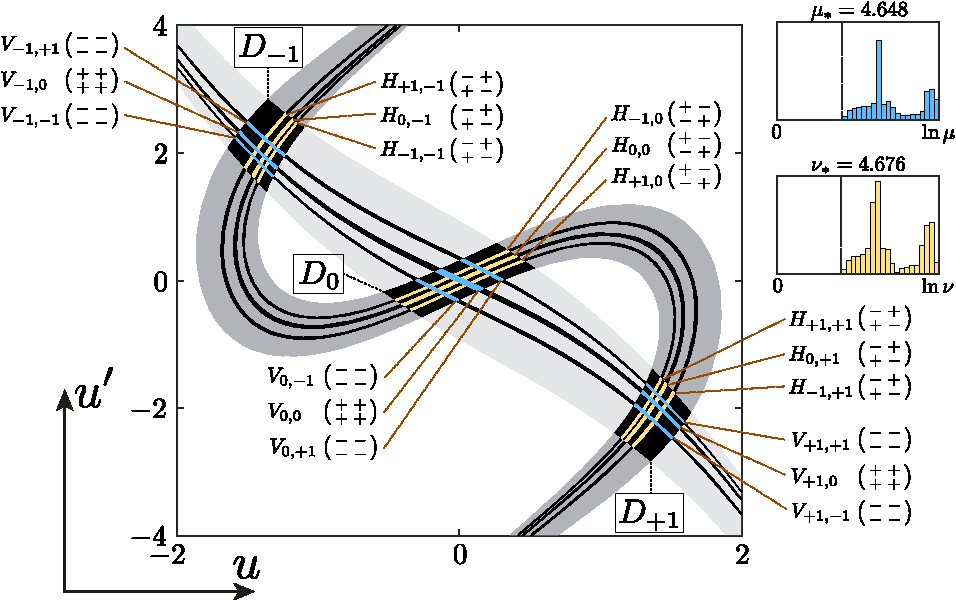
\includegraphics[scale = 1]{../pic/hypotheses for piecewise equation}
	\caption{
		Hypotheses validation for equation \eqref{eq:stationary} for the case $Q(x) \equiv -1$, $P(x) = \eta(x)$ with parameters $(L_*, L_0) = (2, 1)$.
		Set $\mathscr{U}_L^+$ (light gray), $\mathscr{U}_L^-$ (darks gray), and their intersection $\mathcal{D} = \{ D_{-1}, D_0, D_{+1} \} \subset \mathscr{U}_L$ (black) are depicted.
		For the sets $V_{ij}$ (blue) and $H_{ij}$ (yellow) the sings of elements in corresponding operators $D \mathcal{P}_{\vb{p}}$, $D \mathcal{P}_{\vb{q}}^{-1}$ are shown.
	}
\label{fig:hypotheses-validation}
\end{figure}

\textbf{In Chapter III} the set of stationary localized solutions has been studied for the case of equation \eqref{eq:gpe} in which the trapping potential is absent, $U(x) \equiv 0$, and the pseudopotential has a cosine form, $P(x) = A + \cos 2x$.
Such model has been previously considered in literature\textsuperscript{\ref{note:malomed}}.
It was found that this model admits a stationary localized bell-shaped solution, called {\it fundamental soliton}, which is stable for certain parameters of the equation.

In this chapter the coding approach is applied to such model.
Structure of the coding sets is shown in Figure~\ref{fig:island-set}.
In turns out that the sets $\mathscr{U}_{\pi}^{\pm}$ ($L = \pi$) represent infinite spirals which form an unbounded intersection $\mathscr{U}_{\pi}$ consisting of infinite number of connected components.

\begin{figure}[h]
\centering
	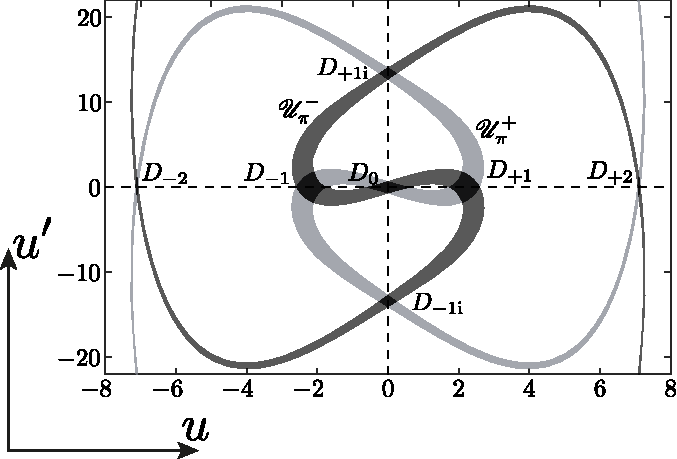
\includegraphics[scale = 1]{../pic/island set to check hypotheses for cosine equation}
	\caption{
		Set $\mathcal{D} \subset \mathscr{U}_{\pi}$ consisting of seven connected components $\{ D_{-2}, D_{-1\mathrm{i}}, D_{-1}, D_0, D_{+1}, D_{+1\mathrm{i}}, D_{+2} \}$ (black), formed by intersection of the sets $\mathscr{U}_{\pi}^{\pm}$ for equation \eqref{eq:stationary} with $Q(x) = -1.5$, $P(x) = \cos 2x$.
	}
\label{fig:island-set}
\end{figure}

Validation of Hypotheses~I and II has been performed numerically for a subset $\mathcal{D} \subset \mathscr{U}_{\pi}$ consisting of seven central connected components.
The numerical procedure allowed to conclude that both of the hypotheses are take place.
Hence, there is a one-to-one correspondence between solutions of equation \eqref{eq:stationary} and symbolic codes derived from the structure of coding set.
Existence of such correspondence allows to conclude that the set of stationary localized solutions of the considered equation is extremely rich.
In Figure~\ref{fig:solutions} different solutions along with their symbolic codes are shown.

Analysis of the linear stability by means of spectral method showed that the majority of solutions are unstable.
However, there is a number of stable solutions, some of which were previously unknown for such model.
One of these new stable solutions is the so-called {\it dipole soliton}.
Its profile is depicted in Figure~\ref{fig:solutions}~(e).
Results of the third chapter were published in \cite{LebedevAlfimovMalomed}, \cite{NizhniNovgorod2016} and \cite{Tashkent2018}.

\begin{figure}[h!]
\centering
	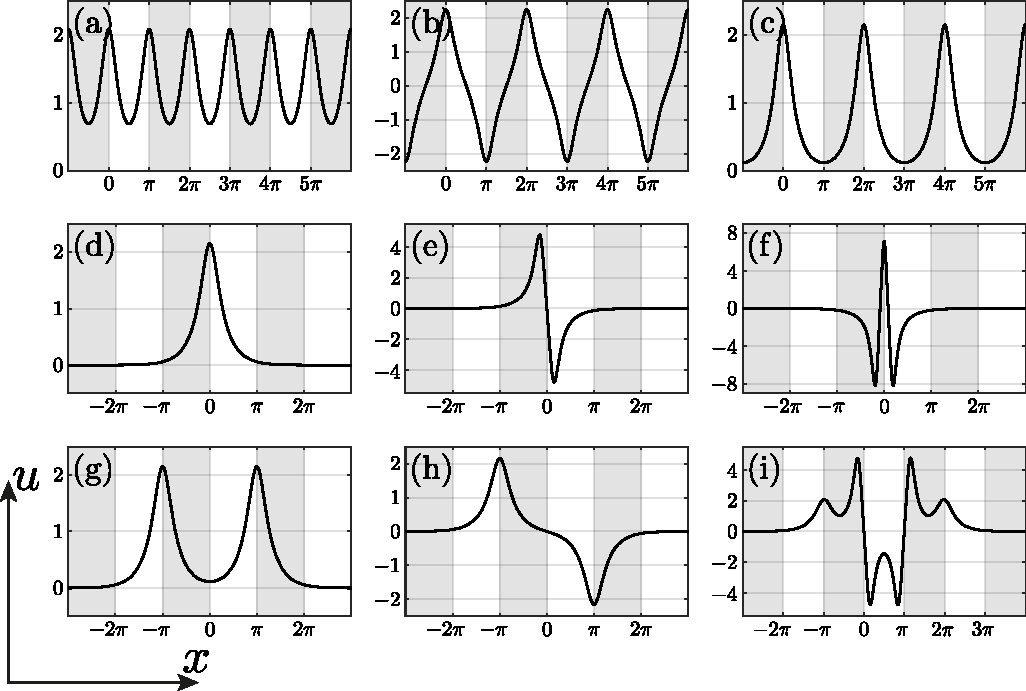
\includegraphics[scale = 1]{../pic/solutions for cosine equation}
	\caption{
		Different solutions of equation \eqref{eq:stationary} for $Q(x) = -1.5$, $P(x) = \cos 2x$.
		Each solution has its own symbolic code that identify the solution uniquely.
		Periodic solutions: (a) $\pi$-periodic solution $\{ \dots, +1, +1, +1, \dots \}$; (b) $2 \pi$-periodic solution $\{ \dots, +1, -1, +1, -1, \dots \}$; (c) $2 \pi$-periodic solution $\{ \dots, +1, 0, +1, 0, \dots \}$.
		Localized solutions (solitons): (d) fundamental soliton $\{ \dots, 0, +1, 0, \dots \}$; (e) dipole soliton $\{ \dots, 0, -1\mathrm{i}, 0, \dots \}$ (f) elementary soliton of code $\{ \dots, 0, +2, 0, \dots \}$ (g) $\{ \dots, 0, +1, 0, +1, 0, \dots \}$ (h) $\{ \dots, 0, +1, 0, -1, 0, \dots \}$ (i) $\{ \dots, 0, +1, -1\mathrm{i}, +1\mathrm{i}, +1, \dots \}$.
	}
\label{fig:solutions}
\end{figure}

\textbf{In Chapter IV} the set of SLMs is studied for equation \eqref{eq:gpe} in which, along with the periodic pseudopotential, there is also a trapping potential of the form of infinite potential well.
After the corresponding renormalization, functions of potential and pseudopotential take forms $U(x) = x^2$, $P(x) = A + B \cos \Omega x$ correspondingly.
Significant place in the analysis of such equation is taken by so-called {\it stationary solutions with a linear counterpart}.
Such solutions arise from the consideration of small-amplitude limit, $|u(x)| \ll 1$.
In this case one can omit nonlinear part in equation \eqref{eq:stationary} and obtain ordinary harmonic oscillator equation,
\begin{equation}
	u_{xx} + (\omega - x^2) u = 0.
\end{equation}
Its solution is the well-known set of eigenvalues and eigenfunctions:
\begin{equation}
	\tilde{\omega}_n = 2n + 1; \quad \tilde{u}_n(x) = \dfrac{1}{\sqrt{2^n n! \sqrt{\pi}}} H_n(x) e^{-\frac{1}{2} x^2}; \quad n = 0, 1, \dots,
\label{eq:ho}
\end{equation}
where functions $H_n(x)$ are Hermite polynomials.
Under action of the nonlinearity each eigenvalue $\tilde{\omega}_n$ bifurcates and originates one-parametric family of solutions $\Gamma_n = (\omega_n, u_n(x))$.
Such families are called as families of solutions with linear counterpart. 

It's known\textsuperscript{\ref{note:alfzez}} that solutions with a linear analogue completely exhaust the entire set of SLMs for the case $P(x) \equiv -1$.
However, in the case of a periodic pseudopotential, there are also exist solutions without linear counterpart.
In this chapter branches of such solution families are constructed numerically, see Figure~\ref{fig:branches}
Linear stability analysis showed that almost all of them are unstable.

The second part of the fourth chapter is devoted to the analysis of the stability for low-amplitude solutions.
It has been analytically shown that in case of zero-mean pseudopotential, $P(x) = B \cos \Omega x$, increase of the frequency leads to stabilization of low-amplitude solutions with linear counterpart.
That is, for each branch $\Gamma_n$ there exists a threshold $\Omega_n$, such that for $\Omega > \Omega_n$ the corresponding solution branch is stable in the vicinity of its bifurcation point $N \ll 1$, $\omega_n \approx \tilde{\omega}_n$.
Results of the fourth chapter were published in \cite{AlfimovGegelLebedevMalomedZezyulin} and \cite{Bannoe2018}.

\begin{figure}[h]
\centering
	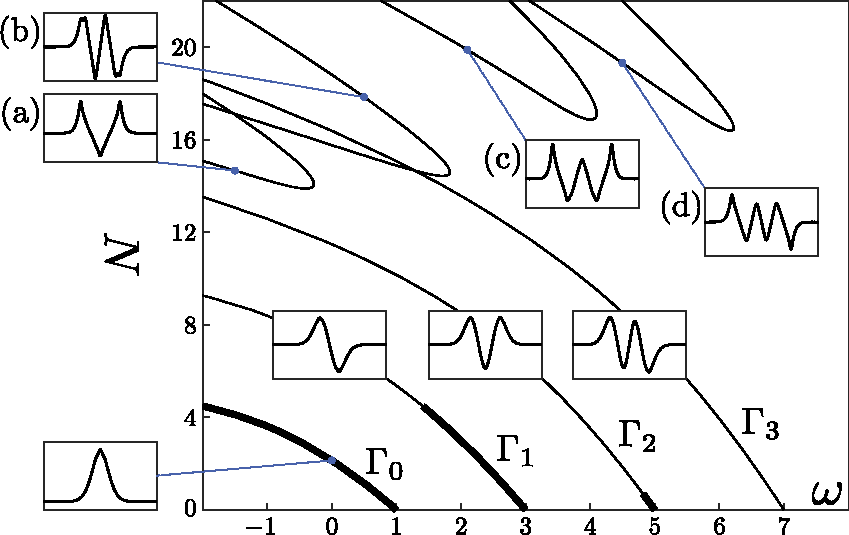
\includegraphics[scale = 1]{pic/branches}
	\caption{
		Diagrams of the dependence of the solutions norm $N$ on the chemical potential $\omega$ for equation \eqref{eq:stationary}; $Q(x) = \omega - x^2$, $P(x) = 1 + 2 \cos (12 x)$.
		Segments of curves $N(\omega)$ that correspond to stable solutions are marked with bold black lines.
		Branches $\Gamma_n$, $n = 0, 1, 2, 3$ correspond to families of solutions with linear counterart.
	}
\label{fig:branches}
\end{figure}

%\begin{figure}[h]
%\centering
%	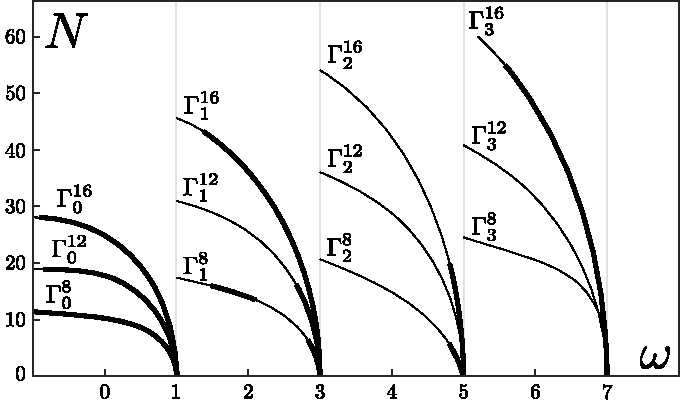
\includegraphics[scale = 1]{pic/branches, different frequencies}
%	\caption{
%		Диаграммы $N(\Omega)$ для ветвей решений с линейным аналогом $\Gamma_n^{\Omega}$, $n = 0, 1, 2, 3$ для уравнения \eqref{eq:stationary}; $Q(x) = \omega - x^2$, $P(x) = \cos \Omega x$, $\Omega = 8, 12, 16$.
%		Сегменты кривых, соответствующие устойчивым решениям, выделены толстыми линями.
%	}
%\label{fig:branches-frequency}
%\end{figure}

\textbf{In Conclusion} the results of the dissertation work are summarized.
The main results can be presented in a following way. 
\begin{enumerate}
	\item General statements about the presence and absence of singular solutions of the equation \eqref{eq:stationary} have been formulated and proved.
	\item Sufficient conditions of coding of regular solutions for equation \eqref{eq:stationary} had been provided.
	An efficient algorithm for the numerical verification of these conditions has been proposed.
	\item For the case $U(x) \equiv 0$, $P(x) = A + \cos 2x$ the set of SLMs for equation \eqref{eq:gpe} has been studied.
	This study revealed new stable localized solution, called {\it dipole soliton}.
	\item In case of infinite potential well is was shown that the presence of periodic pseudopotential leads to the emergence of new classes of SLMs without linear counterpart.
		For the pseudopotential with zero mean, it was found that the increase of pseudopotential frequency can stabilize low-amplitude solutions.
\end{enumerate}

\textbf{In Appendix A} Lemma on bounded solutions is proved.
This lemma is used in Chapter I.

\textbf{Appendix B} contains explicit solutions for two equations of the Duffing oscillator type: 
\begin{equation}
	u_{xx} - u + u^3 = 0; \quad u_{xx} - u - u^3 = 0.
\end{equation}

\textbf{In Appendix C} Theorems on h- and v-strips mapping are proved.
These theorems are used in Chapter II.

% \renewcommand{\bibname}{\protect\leftline{Bibliography}}

\def\thispagestyle#1{}
\renewcommand{\bibname}{\protect\leftline{\large List of Publications on the Topic of Dissertation}}
\printbibliography[keyword=own]

% Center aligned bibliography title
% \printbibliography[keyword=own, title={\large Список публикаций автора по теме диссертации}]

% All other cited literature
% \printbibliography[notkeyword=own, title={Цитированная литература}]

\end{document}
